% Translated from sections/03-corpus-and-system.tex on 2026-09-23. The English
% file is canonical. Change it first, then carry the change here.
%
% The plates are illustrative, not measured, exactly as in the English file.
\section{Corpus et système}
\label{sec:corpus}

Deux ensembles d'imprimés français du \sxvi, qui ne sont pas indépendants.
\emph{Amadis de Gaule} est un cycle de romans de chevalerie en \ocrBooks{}~livres,
soit \ocrPages{}~pages numérisées. Les anthologies du \emph{Trésor} reprennent
des extraits de ce cycle sous des rubriques thématiques. Localiser une pièce du
\emph{Trésor} est donc une tâche de recherche dont la réponse est vérifiable. La
spécification de conception traite les deux œuvres comme un seul domaine cible.
Rien de ce qui suit n'oppose un domaine connu à un domaine étranger.

\begin{figure}[t]
  \centering
  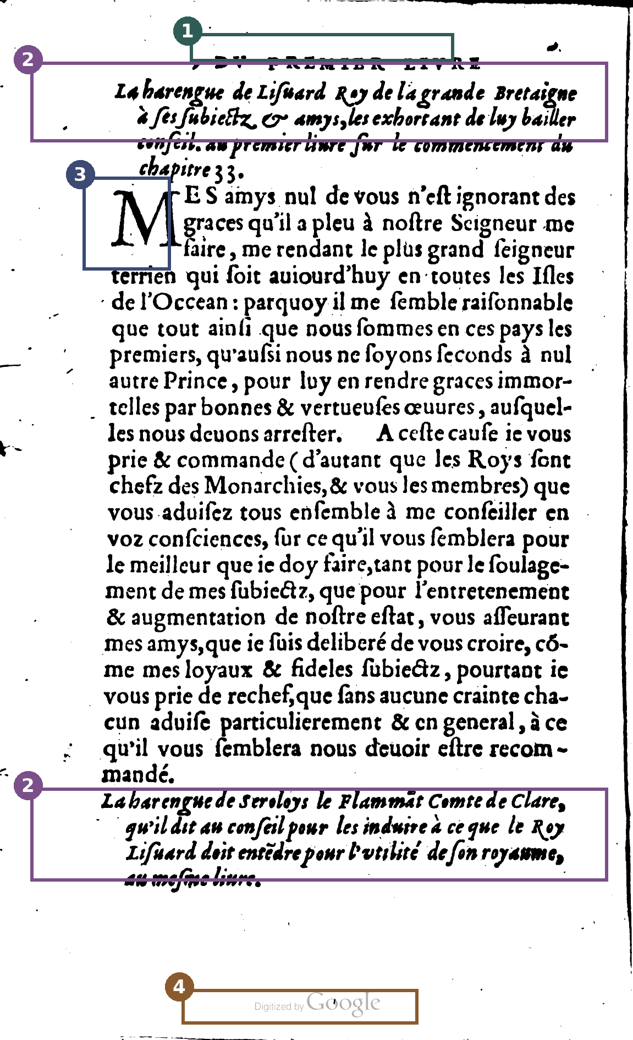
\includegraphics[width=0.62\linewidth]{plates/page-thresor.png}
  \caption{Une page du \emph{Thresor des douze livres d'Amadis de Gaule}
    (1559), le volume sur lequel le modèle livré a été affiné. \textbf{1}
    titre courant, \qtr{DV PREMIER LIVRE}. \textbf{2} rubriques en italique,
    promues en titres par leur inclinaison et non par leur libellé. \textbf{3}
    la lettrine \qtr{M} de \qtr{MES amys}, que la segmentation en lignes ne
    voit pas. \textbf{4} le filigrane du numériseur, repéré comme candidat pied
    de page et exclu de la transcription. \qtr{ſ} long partout. Annotations
    ajoutées pour cette figure.}
  \label{fig:plate}
\end{figure}

\subsection{Deux éditions, trois provenances}

Les \ocrBooks{}~livres ne forment pas une seule édition. Les
\ocrBooksFamilyA{}~premiers (famille~A) sont de grand format, en
\emph{bâtarde}, foliotés en chiffres romains, et chaque volume s'ouvre sur une
table des matières imprimée. Les \ocrBooksFamilyB{}~autres (famille~B) sont
plus tardifs et plus petits, en romain net avec des rubriques en italique, une
pagination en chiffres arabes et aucune table des matières. La famille~A
compte \ocrPagesFamilyA{}~pages, la famille~B \ocrPagesFamilyB{}. La
reconnaissance est donc rapportée par famille. La calibration structurelle ne
couvre que la famille~A, parce qu'il lui faut une table des matières imprimée
à laquelle se comparer. Le débit regroupe les deux, car chaque livre a été
traité par un même modèle, sur un même matériel, à une même largeur de travail.

Trois institutions de conservation, trois états. Le livre~1 est en TIFF
bitonal à 600~dpi de la Bibliothèque municipale de Lyon, les livres~3 et~4 en
PDF en niveaux de gris de Gallica, et le livre~18 un exemplaire de la
Biblioteca Valenciana qui porte le tampon de cette bibliothèque. La provenance
des autres volumes n'est consignée nulle part et n'est pas affirmée ici. La
provenance introduit une variation sans rapport avec le siècle. La
section~\ref{sec:protocol} stratifie donc selon ce critère.

\subsection{Les pièces du \emph{Trésor}, et le corpus d'entraînement}

La référence est le catalogue de l'éditeur,
\file{data/localisation/ground-truth.csv}. Il compte \corpusPieces{}~pièces,
chacune avec un Livre et, quand l'imprimé en donne un, un chapitre. C'est une
prose écrite par un érudit, et la transcription en conserve les réserves.
\corpusCertain{}~pièces (\corpusCertainShare{}) portent une attribution sans
réserve. \corpusUncertain{} sont suivies d'un point d'interrogation,
\corpusConjecture{} sont des conjectures entre crochets et \corpusUnassigned{}
ne nomment aucun emplacement. Seules les attributions certaines sont évaluées.
L'apparieur a placé \corpusAligned{}~pièces, tirées de \corpusLivres{} des
\ocrBooks{}~livres, d'une longueur médiane de \corpusCharsMedian{}~points de
code et de \corpusCharsMax{} au plus.

Deux lots, séparés partout. La cohorte classeur compte
\corpusPiecesWorkbook{}~pièces. C'est le lot qui existait quand la règle de E5
a été préenregistrée. La cohorte catalogue compte \corpusPiecesCatalogue{}~pièces,
importées quatre jours plus tard. Les regrouper reviendrait à agrandir un jeu
de test après en avoir vu les chiffres.

Le corpus d'entraînement compte \trainPages{}~pages annotées, toutes issues
d'une même collection Transkribus, \emph{Trésor des Amadis}~T.1.
\trainPagesTrain{} servent à l'entraînement et \trainPagesVal{} sont réservées.
Les pages réservées sont une validation et non un test, puisqu'elles ont servi
à choisir le point de contrôle livré. Les deux familles d'\emph{Amadis de
Gaule} sont donc en grande partie inconnues du modèle qui les a transcrites. La
section~\ref{sec:limitations} dit ce que coûte ce découpage.

\subsection{La chaîne de traitement}
\label{sec:system}

\begin{figure}[t]
  \centering
  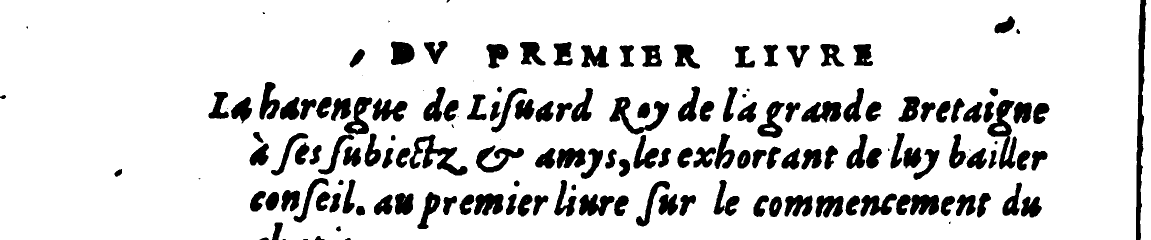
\includegraphics[width=0.86\linewidth]{plates/spec-rubric.png}\\[0.35em]
  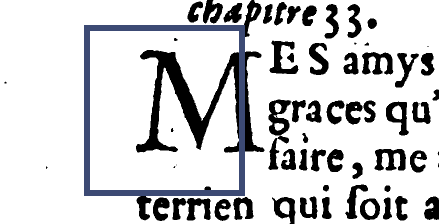
\includegraphics[width=0.33\linewidth]{plates/spec-dropcap.png}\hfill
  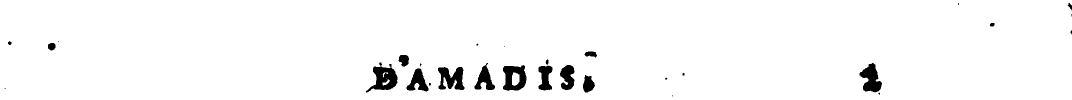
\includegraphics[width=0.60\linewidth]{plates/spec-header.png}
  \caption{Ce que regarde l'étape de mise en page, qui n'est que géométrie. En
    haut, le corps du texte est proche de $0^\circ$ et cette rubrique penche
    de 12 à 18$^\circ$, mesurés par rapport à l'inclinaison médiane du corps de
    la page. C'est l'inclinaison qui signale un titre, jamais le libellé. En
    bas à gauche, une tache d'encre de 1,6 à 9~fois la hauteur de ligne, d'un
    rapport d'aspect entre 0,4 et 1,8, dans les 20\,\% gauches de la colonne,
    est une lettrine. En bas à droite, une ligne courte et centrée portant un
    numéro de folio est un titre courant.}
  \label{fig:layout}
\end{figure}

La reconnaissance est assurée par kraken~7.0.2 \cite{kiessling2025kraken},
avec un modèle affiné à partir de CATMuS-Print [Large]
\cite{gabay2024catmusprintlarge} sur les \trainPages{}~pages décrites plus
haut. L'artefact livré est \file{amadis-ft.mlmodel}. Son empreinte SHA-256
figure dans \file{PROVENANCE.md}, et la comparaison des poids le rattache au
point de contrôle d'entraînement dont il est issu. Deux configurations ont été
exécutées. Celle qui a été livrée suit un calendrier de réduction sur plateau
avec un taux d'apprentissage de $3\times10^{-4}$ et de l'augmentation de
données. Une exécution antérieure à taux constant de $10^{-3}$ n'a pas été
livrée.

La mise en page est déterministe et ne comporte aucun composant appris
(figure~\ref{fig:layout}). Les bandes de lignes de base donnent l'ordre de
lecture. Les lignes trop grandes ou inclinées comme l'italique deviennent des
titres. Les lignes des marges haute et basse deviennent des titres courants et
des pieds de page. Les zones d'illustration et les tampons de bibliothèque
sont écartés au lieu d'être lus. Ce qu'elle ne peut trancher, c'est le cas
ambigu d'une ligne isolée en haut ou en bas de page qui peut être un titre
courant, une réclame, ou la première ou dernière ligne du corps. Ce résidu est
ce que E3 évaluerait.

Deux passes par LLM suivent la reconnaissance. Toutes deux sont facultatives,
toutes deux s'exécutent après la reconnaissance, et toutes deux reviennent à
\emph{ne rien changer} quand le modèle est absent ou échoue. La \textbf{passe
de cohérence} tranche une ligne de tête ou de pied ambiguë en demandant si sa
suppression laisse les lignes voisines se lire d'un seul tenant. La
\textbf{passe de faible confiance} est l'objet de l'affirmation~C2. Chaque mot
contenant un caractère noté sous \texttt{LOWCONF\_THRESHOLD} est entouré de
\lmark~\rmark{}, et la ligne est envoyée avec ses deux voisines pour contexte,
la consigne interdisant toute orthographe modernisée. La réponse est découpée
selon les marqueurs. Elle n'est acceptée que si le nombre de marqueurs
concorde et si chaque segment situé \emph{hors} des marqueurs est identique à
l'original, octet pour octet. Sinon la ligne entière revient à son état
initial. Il n'y a pas d'acceptation partielle. Cette règle est le cœur de la
contribution. Elle rend une réécriture structurellement détectable au lieu de
plausible, et donc refusable.

La localisation est une recherche sur la transcription complète des
\ocrBooks{}~livres. Un normaliseur attentif à l'époque replie la variation
orthographique qui ferait échouer une correspondance exacte. Un index
d'amorces propose des positions candidates. Les amorces sont les mots rares,
d'au moins \texttt{MIN\_SEED\_LENGTH}~caractères et d'une fréquence
documentaire d'au plus \texttt{MAX\_SEED\_DF}. Un chaînage d'ancres par livre
les assemble en une étendue, acceptée si son score dépasse
\texttt{MIN\_SCORE}.

\begin{table}[t]
  \centering
  \begin{tabular}{llll}
    \toprule
    Constante & Valeur & Origine & Balayée ici \\
    \midrule
    \texttt{LOWCONF\_THRESHOLD}    & 0,6   & relevée de 0,5 à la main & non \\
    \texttt{OCR\_DROPCAP\_MIN\_PROB} & 0,6   & défaut, jamais balayée & non \\
    \texttt{MIN\_SCORE}            & 0,808 & plancher observé        & vérifiée, \S\ref{sec:e5} \\
    \texttt{MIN\_SEED\_LENGTH}     & 6     & défaut                  & non \\
    \texttt{MAX\_SEED\_DF}         & 200   & défaut                  & non \\
    \texttt{UNCERTAIN}             & 0,85  & seuil de relecture      & non \\
    \bottomrule
  \end{tabular}
  \caption{Les six constantes dont dépend le comportement du système. Ce
    rapport en calibre une. Les autres sont héritées et sont nommées pour que
    rien ne repose sur elles en silence. \texttt{CHAIN\_GAP\_PENALTY} et
    \texttt{WINDOW\_SLACK} n'y figurent pas, parce qu'elles n'ont jamais été
    modifiées non plus.}
  \label{tab:thresholds}
\end{table}

Le tableau~\ref{tab:thresholds} recense tous les seuils que contient le
système. Cinq des six ont été choisis à la main ou laissés à leur valeur par
défaut, et n'ont jamais été balayés.
